\documentclass[12pt]{report}
\usepackage[dvips]{graphicx}
\usepackage[utf8]{inputenc}
\usepackage{color}
\usepackage{times}
\usepackage{tabularx}
\usepackage{multirow}

\title{TrafDump v.123}
\author{Eugeni Dodonov\footnote{eugeni@dodonov.net} \and Paulo Costa\footnote{paulov.x.costa@intel.com}}
\date{\today}

\begin{document}

\maketitle

\begin{abstract}

This documents outlines main features, installation proceedings and known problems for TrafDump.

\end{abstract}

\tableofcontents

\chapter{Project overview}

TrafDump was designed as a network evaluation benchmark application, aiming at
identifying bottlenecks, network environment constraints and limitations,
and providing comprehensive and complete results.

The application supports the following modes of operation:

\begin{itemize}

\item \textbf{Quick Test} -- this performs a quick test of the environment,
evaluating only the multicast capabilities for $400$, $800$, $1200$, $1600$
and $2000$ Kbps transfers. After the test, a PDF report is generated with
overall results;

\item \textbf{Full Test} -- this performs a full test of the environment,
evaluating the TCP throughput for each client, multicast capabilities for
bandwidth from $400$ up to $4000$ Kbps, with step of $100$ Kbps. The
resulting PDF report contains both the overall and detailed results for each
test.

\item \textbf{Estimate TCP} -- this runs the TCP Throughput test, estimating
both the upload and download capabilities of the clients.

\item \textbf{Estimate multicast} -- this runs a multicast test, estimating
the reception quality (message loss), and sustained transfer rate. This test
can be performed for both individual bandwidths (such as, for example,
$1000$ Kbps), and for bandwidth interval (for example, from $1000$ to $2000$
Kbps, with step of $100$ Kbps).

\item \textbf{Estimate broadcast} -- this is essentially the same as the
multicast test, with the difference that broadcasting messages are used
instead of multicast ones.

\item \textbf{Wireshark integration} -- this allows a more detailed
evaluation of the environment, by running a wireshark application on each
client for traffic analysis. After the execution, and resulting files are
retrieved for posterior analysis. If wireshark is not installed on the
clients, this does nothing.

\begin{figure}
\centering
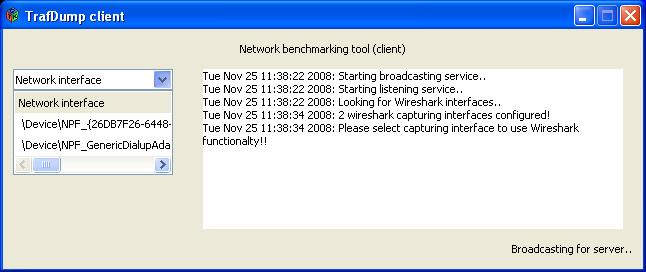
\includegraphics[scale=0.7]{netwin.JPG}
\label{f:netwin}
\caption{Trafdump client interface: network card selection}
\end{figure}

Note that in order to use wireshark, it is necessary to select the
network card for the capturing, as shown on figure \ref{f:netwin}. If
wireshark is not installed, or the user has no privileges to perform traffic
capturing, the options is not available and the network card selection
box is disabled (figure \ref{f:netlin}).

\begin{figure}
\centering
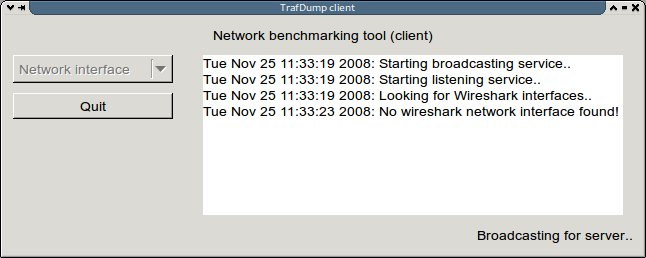
\includegraphics[scale=0.5]{netlin.jpg}
\label{f:netlin}
\caption{Trafdump client interface: traffic capture not available}
\end{figure}

\end{itemize}

For each test, different sets of client machines can be selected. By default, when
a client connects to the trafdump application, it is selected. To deselect a
client, simply click on its icon. Active clients are marked as blue, and
inactive as black, as shown on figure \ref{f:clients}.

\begin{figure}[h!t]
\centering
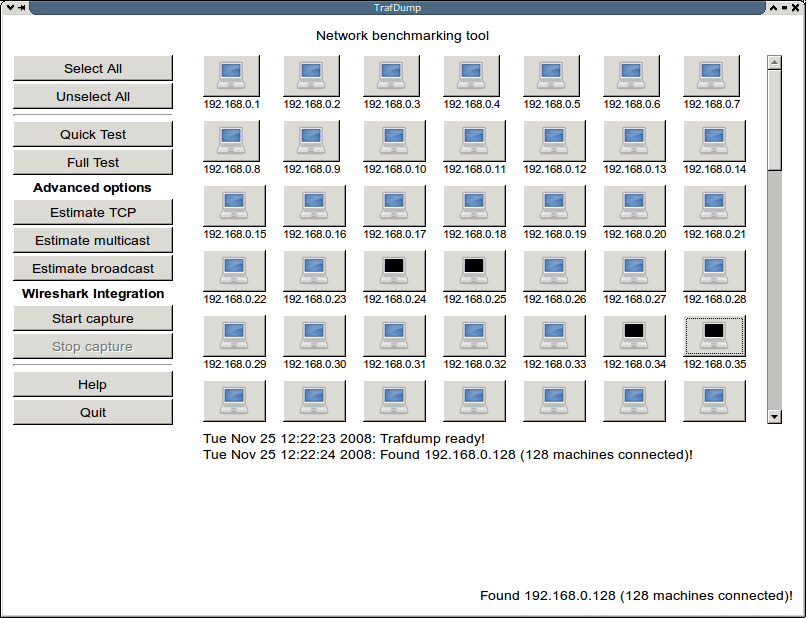
\includegraphics[scale=0.5]{clients.png}
\label{f:clients}
\caption{Trafdump interface: client selection}
\end{figure}

In case of a network communication failure with one of the clients, its
state will automatically change to deselected. If mouse is passed over its
icon, a short message will appear with the description of last communication error.

The results of all experiments are saved into independent directories, named
according to the experiment description plus a time stamp (for example,
\textbf{Quick experiment.122827281}). This allows running different
experiments with the same name. Among with PDF reports, individual results
in PNG and CSV format are also saved and can be used for detailed
evaluation.

\chapter{Installation}

TrafDump was developed in a cross-platform way, with the goal of covering
the most widely available platforms. Currently, the application is supported
on Microsoft Windows and Linux environments, running at least on a pentium-3
$500$ MHz with $256$ MB of RAM.

The application was written in \emph{python}
\footnote{http://www.python.org/} $2.5$, but it is also known to work with
\emph{python} $2.4$ and $2.6$. Graphical interface was written in
\emph{PyGTK} \footnote{http://www.pygtk.org/}, using \emph{GTK} toolkit
\footnote{http://www.gtk.org/}. Chart are created using \emph{Matplotlib}
\footnote{http://matplotlib.sourceforge.net/}, and PDF reports are generated
with \emph{ReportLab} \footnote{http://www.reportlab.org/} libraries. If you
intend to use the traffic capturing capabilities of the application, it is
also necessary to install the \emph{WireShark}
\footnote{http://www.wireshark.org/} application. Please note that the
\emph{Wireshark} uses additional $90$ MB of disk space, and delays the
startup of client application by a few seconds. Therefore, we do not
recommend the usage of this application for production use.

Binary version of TrafDump includes all the necessary libraries in a compact
way. Therefore, while the binary distribution of TrafDump requires $35$ MB
disk space, the installation of all libraries would require more that $180$
MB. The installation of libraries is only required when using source version
of the application.

TrafDump is distributed in two versions: one compacted with \emph{7zip}
\footnote{http://www.7zip.org/}, and using a common \emph{ZIP} file. The
\emph{7zip} version is recommended, as the distribution file is roughly $50\%$
smaller. Also, two different packages are available: \emph{client.zip} and
\emph{client.7z}, which contain only the client application, while
\emph{trafdump.zip} and \emph{trafdump.7z} where both client and main
application are included.

To use the application, uncompress the distribution files, and execute
\emph{trafdump.exe} on server machine, and \emph{client.exe} on each
client. When using source version, the corresponding files are
\emph{trafdump.py} and \emph{client.py}.

In order to allow communication between main application and clients,
certify the following ports are open in your firewall:

\begin{itemize}

\item \textbf{TCP port 10000}: used for communication between clients and
the main application;

\item \textbf{UDP port 10000}: used for clients discovery;

\item \textbf{UDP port 10001}: used for multicast experiments;

\item \textbf{UDP port 10002}: used for broadcast experiments.

\end{itemize}

\chapter{Known issues}

The following issues are known in this version of TrafDump:

\begin{itemize}

\item When clients go offline, the main application won't detect it until
next experiment. This will be fixed in future versions.

\item Detailed experiment description (such as the wireless parameters, user
name, and additional user notes) is not available in this version. This will
be fixed in future versions.

\item When many clients are used for an experiment, the resulting PDF file
may contain very long text lines. This will be fixed in future versions.

\item Very big charts may result in low readability. This will be fixed in
the next versions.

\item After an experiment is finished, resulting graphics or PDF files are
not automatically displayed. This will be fixed in the next versions.

\item (Linux) if main application window loses focus, or when no mouse or
keyboard activity is performed for a long time, the window may stop being
refreshed. To work around this problem, simply move the mouse. This will be
fixed in the next versions.

\item (Linux) if the current user doesn't have the writing permissions to
the directory where client is running, tshark application won't be able to
capture traffic, even when running by root user. This can be temporarily
solved by running "chmod 777 ." on a current directory, or changing the
directory owner to root.

\end{itemize}

\end{document}
